%
\documentclass[Journal]{ascelike}
%
% Feb. 14, 2013
%
% Some useful packages...
%
\usepackage{adjustbox}
\usepackage{graphicx}
%\usepackage{subfigure}
\usepackage{amsmath}
\usepackage{amsfonts}
\usepackage{amssymb}
%\usepackage{amsbsy}
%\usepackage{times}
\usepackage{color}
\usepackage{listings}
\usepackage{subcaption}
\usepackage{nameref}
\usepackage{rotating}
\usepackage{pdflscape}
%
% Place hyperlinks within the pdf file (works only with pdflatex, not latex)
% \usepackage[colorlinks=true,citecolor=red,linkcolor=black]{hyperref}
%
%
% NOTE: Don't include the \NameTag{<your name>} if you have selected 
%       the NoPageNumbers option: this leads to an inconsistency and
%       a warning, and the NameTag is ignored.
%\NameTag{Nam Lethanh, April. 02, 2014}
%
%
\begin{document}
%% You will need to make the title all-caps
\title{Determination of Markov Transition Probabilities to be used in Bridge
Management from Mechanistic-Empirical Models}%
\author{
Nam Lethanh\thanks{PhD. Principal, InfraPlus, 2001B-C1-Ecopark, HungYen, Vietnam. E-mail: namlt@protonmail.ch}, J\"{u}rgen Hackl\thanks{PhD Candidate, Institute of Construction and Infrastructure Management,
Swiss Federal Institute of Technology (ETH), Z\"{u}rich 8093, Switzerland. E-mail: hackl@ibi.baug.ethz.ch} and Bryan T. Adey%
\thanks{PhD. Institute of Construction and Infrastructure Management., Swiss Federal 
Institute of Technology (ETH), 8093 Z\"{u}rich, Switzerland. E-mail: adey@ibi.baug.ethz.ch}\
}
%
\maketitle
%
\begin{abstract}
Reinforced concrete elements of a bridge deteriorate due to chloride
induced corrosion. This process can be modeled using two mechanistic-empirical
models. The first is to model deterioration in the initiation phase,
which is when there chloride ions infiltrate into the concrete but
there is no corrosion of the reinforcement. The second is used to
model deterioration in the propagation phase, when there is corrosion
of the reinforcement. Mechanistic-empirical models such as these are
used extensively to investigate the detailed behavior of reinforced
concrete structures.In managing reinforced concrete bridges, instead
of using mechanistic-empirical models Markov models are often used.
They are used to predict the deterioration of large numbers of similar
objects, which is subsequently used in the determination of optimal
intervention strategies and intervention programs. Markov models are
used because the effort of using mechanistic-empirical models on all
objects would be an immense effort for which there may be minimal
benefit. Markov models can be developed immediately, using the results
of visual inspections, which are regularly conducted and stored in
databases anyway, or will be regularly conduced in the future. In
situations where visual inspections have not been regularly conducted
or the results have not been stored in a database, it would be useful
to estimate the transition probabilities to be used in the Markov
models using mechanistic-empirical models. In the investigation presented
in this paper a new methodology was developed to to do this. , i.e.
to estimate the transition probabilities to be used in Markov models
to predict the deterioration of reinforced concrete bridges. The transition
probabilities are estimated using a restricted least squared optimization
model that ensure the closest fit between the distribution of condition
states predicted using the Markov model and predicted using the mechanistic-empirical
models, i.e. proportional data. The methodology is demonstrated by
estimating the optimal transition probabilities for a reinforced concrete
bridge deck. 
\end{abstract}
%
% Some keywords, using a new command: \KeyWords{}
%
\KeyWords{Mechanistic-Empirical Corrosion Models; Markov Models; Reinforced Concrete Bridges; Simulation.}
%


\section{Introduction}

\label{introduction} 
In many existing bridge management systems , the deterioration of
reinforced concrete bridge elements is modeled using Markov models.
Markov models are stochastic models, which define the space of physical
condition of the elements into a range of discrete condition states.
Markov models are used because the effort of using mechanistic-empirical
models on all objects would be an immense effort for which there may
be minimal benefit. Markov models can be developed immediately, using
the results of visual inspections, which are regularly conducted and
stored in databases anyway, or will be regularly conduced in the future.
In situations where visual inspections have not been regularly conducted
or the results have not been stored in a database, it would be useful
to estimate the transition probabilities to be used in the Markov
models using mechanistic-empirical models. Situations where there
might be inadequate data include 1) lack of data because the infrastructure
is newly built or in the past the inspection results have not been
archived, 2) inconsistent data in time due to inconsistently conducted
monitoring programs, 3) biased data, due to lack of strict guidelines
for inspector, and 4) data with large errors, due faulty measurement
equipment. 

Using Markov models in this situation, the evolution of condition
of the elements over time is expressed by means of a time dependent
state vector, which is calculated using a transition probability matrix.
The accurate estimation of the transition probabilities to be used
in the Markov model affects the prediction of the future condition
of bridge element, which can affect the determination of the optimal
intervention strategies for the elements and in turn the development
of the intervention program to be implemented. 

In regard to the estimation of transition probabilities, currently,
statistical models of the length of time of how long an element remains
in a condition state are often derived from a set of time-series inspection
data. The inspection data is usually that collected via visual inspections
and the condition states are usually defined with values of a composite
index. In the estimation of the transition probabilities it is either
assumed that the probabilities of transitioning more than one condition
state in one unit of time is zero, and therefore only the probabilities
of transitioning one condition state in one unit of time need to be
estimated \cite{Klein1962,Camahan1987}, or that it is possible to
transition from one condition state to all other higher condition
states and then all probabilities of transition are estimated. There
are numerous ways to estimate the transition probabilities when data
has been collected at constant time intervals. There are a smaller
number of ways to estimate the transition probabilities when data
has been collected at non-constant time intervals, of which one is
\cite{Tsuda2006,Kobayashi2012}.

In the situations where there is inadequate data in terms of quantity
or quality, to accurately estimate the transition probabilities to
be used in Markov model, it is useful to be able to estimate them
using mechanistic-empirical models, which was first tried in \cite{Roelfstra2004}.When
mechanistic-empirical models are used to model. It is possible to use
mechanistic-empirical models to model the deterioration process of
reinforced concrete elements in these situations because they can
be based on the characteristics of the element, including material
properties, location, and environment, which can be tested. One of
the challenges of estimating the transition probabilities from mechanistic-empirical
models is that the they predict condition evolution on continuous
scales, and the transition probabilities are between discrete states
\cite{DuraCrete1998}.

In this paper, a new methodology is presented to estimate the transition
probabilities for reinforced concrete bridge elements that are affected
by chloride induced corrosion of the reinforcement using mechanistic-empirical
models. In the methodology, the mechanistic-empirical model and statistical
values of the model's parameters are first used to generate proportional
data on discrete states of the bridge elements over time using Monte
Carlo simulations, and this data is then used in a restricted constraint
optimization model to estimate the transition probabilities. The methodology
is demonstrated by estimating the optimal transition probabilities
for the elements of a reinforced concrete bridge.

\section{Estimation of transition probabilities using inspection data}
\label{mdpd} 

As long as discrete state Markov models have been used, it has been
necessary to estimate the probabilities of transition between the
states. This is necessary to estimate the evolution of the condition
over time. When inspection data is available, this has been done in
numerous ways, from simple to complex, with varying degrees of accuracy.
The simplest way is the division of the number of elements that have
made transitions in the past by the total number of elements \cite{Tsuda2006},
and one of the more complex ways is that proposed by \citeN{Tsuda2006}
and \citeN{Kobayashi2012}, in which likelihood estimation approach
or Bayesian estimation approach are used to derive the optimal value
of transition probabilities. The former works, however, only when
the inspection data has been collected at regular intervals. The later
works even if the inspection data has not been collected at regular
intervals. In some situations, researchers and practitioners have
simplified the estimation of transition probabilities by assuming
that an element cannot transition more than one state per unit time\cite{Jiang1988,Al-Subhi1989,Mishalani2002,Robelin2007} Although convenient from a mathematical perspective, it would be beneficial
if this assumption was not, or did not have to, be made. This assumption
is not required with the ways proposed by \citeN{Tsuda2006} and \citeN{Kobayashi2012}.

\section{Estimation of transition probabilities without using inspection data }

When there is insufficient inspection data to estimate transition
probabilities directly other methods are required. These range from
using expert opinion to estimating the transition probabilities so
that there is the closest correlation possible with the results of
mechanistic-empirical models.

Mechanistic empirical models are used extensively to estimate the reliability
of specific reinforced concrete bridge elements \cite{DuraCrete1998,Kirkpatrick2002}.
These models have a wide range of forms, e.g. linear, exponential.
They are usually developed with a solid understanding of the processes
at work in the reinforced concrete elements, insights provided by
laboratory or in-situ tests, and data collected to evaluate the actual
state of the bridge element. Mathematically, a ME model is defined
as functions of a set of parameters. For example, the level of chloride
is a function of time, initial level of chloride ion concentration,
the distance of re-bars from concrete surface, and chloride diffusion
coefficient \cite{Kirkpatrick2002}. When values of parameters are
determined, the continuous evolution of deterioration indicator (e.g.
level of chloride over time) can be straightforward visualized. In
order to include the uncertainty in deterioration prediction, parameters
of mechanistic-empirical models are represented with probabilistic
distributions (e.g. normal distribution, log-normal distribution). 

One of the most widely supported mechanistic empirical models is the
one proposed by \cite{DuraCrete1998,Kirkpatrick2002}. This model
enables estimates of when the duration of the initiation phase in
which chloride ions penetrate into the concrete and break down the
passivisation layer on the reinforcement and the estimation of the
length of the propagation phase, in which corrosion occurs until a
specific section loss threshold is reached . They have also made proposals
as to the distributions to be used in the estimation of the parameter
values \cite{DuraCrete2000}.

When mechanistic-empirical models are used to estimate transition
probabilities a decision has to be made as to how one will determine
that there is indeed a good fit with deterioration predicted using
the resulting Markov model and the deterioration predicted using the
mechanistic empirical model. One of the first work in the area is
that of \citeN{Roelfstra1999} and \citeN{Roelfstra2004} who assumed
that each element could transition no more than one state in one unit
of time and obtained a best fit using least squares estimation approach.
The best fit was determined as being the transition probabilities that
gave the least error between the average condition states in each
of the investigated time period predicted by the Markov model and
predicted by the mechanistic-empirical model. The validity of the
assumption of not transitioning more than one state in one unt of
time depends on the speed of deterioration, but it is an assumption
made by many researchers \cite{Jiang1988,Al-Subhi1989,Mishalani2002,Robelin2007}
and used in the past for the estimation of transition probabilities
for use in bridge management systems such as the Pontis \cite{pontis,Soderqvist1998,Thompson1998,Thompson1999a,FHWA2002} and the KUBA-MS \cite{Hajdin2003,Hajdin2006}.

Another way to establish a best fit between the models is to minimize
the errors between the probability of being in each state in each
time interval in the investigated period predicted using the Markov
model and the mechanistic empirical model, instead of just the average.
Although computationally more intensive this should give more detailed
and better approximations of the future behavior of the elements.
This can be done by first estimating the probable values of the deterioration
indicators such as level of chloride concentration or the width of
crack, in each time interval and summarized as a state vector, i.e.
at time $t+1$, there is a probability of being in each state i. This
type of data is referred to as proportional data.

Although the use of proportional data to estimate transition probabilities
has not been used in the field of bridge management, there has been
substantial early work in the fields of econometrics and financial
engineering \cite{Lee1972}. As summarized in \citeN{toukei}, it
started in the 1950s when \citeN{Miller1952} proposed a discrete
Markov processes in psychology. He defined a stochastic relation formulation
as a basic for describing a linear statistical model for estimating
the transition probabilities from proportional data using an unrestricted
least squares transition probability estimator. Later, a restricted
least squares transition probability estimator was developed by \citeN{Goodm1953}
. Since then, there has been a significant amount of research done
on improving the the estimation of transition probabilities. Many
of these have concentrated on the use of the maximum likelihood estimation
and Bayesian estimation approaches \cite{Lee1972,lancaster90,Kobayashi2012}.

The methodology presented in this paper uses proportional data generated
from mechanistic-empirical models to estimate the transition probabilities
for reinforced concrete bridge elements .

\section{Methodology}
\label{methodology}
The methodology is shown in Figure \ref{methodoframe}. The first
two tasks are to select the mechanistic empirical models to be used.
Once the models are selected, the values of their parameters are defined,
for example, using the standard codes defined in \citeN{DuraCrete2000}.
Using these values, the values of the condition indicators at every
future time are randomly generated. Simultaneously, a range of condition
states used to map the continuous values emanating from the mechanistic-empirical
models are defined. Once these steps are complete, the values of the
indicators at every time steps are used to determine the state of
the element. The distribution of these probable condition states in
each time interval is referred to as proportional data. The transition
probabilities are then estimated using the restricted least-squared
optimization model to minimize the errors between the distributions
obtained using the proportional data and the distributions obtained
using the Markov model over the entire investigated time period. Finally,
an evaluation of the transition probabilities is conducted by examining
how the element is to deteriorate over the investigated time period
and the values of error terms. Each task is explained in more detaile
in the following sections.

\begin{figure}[h!]
\centering \includegraphics[scale=0.6]{framework} \caption{Methodology}
\label{methodoframe} 
\end{figure}

\subsection{Task 1: Develop mechanistic-empirical models}

A mechanistic model is one that is based on the physical behavior
of the elements in the system. An empirical model is one that is based
on direct observation, measurement and extensive data records, often
without understanding the physical behavior of the element in the
system. A mechanistic- empirical model is a combination of both. These
types of models are often used to predict the occurrence of very specific
conditions, e.g. the amount of chlorides at a specific depth in a
concrete beam. Coupled with the probabilistic distributions to represent
the values of the variables and parameters in the models, they can
be used to estimate the probable specific conditions. For reinforced
concrete elements, a widely used mechanistic-empirical model to model
the chloride induced corrosion of the reinforcement is the one proposed
by \citeN{DuraCrete1998} and \citeN{Roelfstra2004}. This deterioration
process can be divided into two phases, the the initiation phase,
in which chlorides penetrate into the concrete and corrosion starts
but has not yet progressed to the point where there are any corrosion
induced cracks at the surface, and the cracking phase, in which cracks
grow. The deterioration process is illustrated in Figure \ref{fig1}.

\begin{figure}[h!]
\centering \includegraphics[scale=0.4]{twophases} \caption{Deterioration process of reinforced concrete due to chloride-induced corrosion.}
\label{fig1} 
\end{figure}

In the figure, additional information such as condition states (CS1,
CS2, CS3, CS4, and CS5) are given along with the range of chloride
concentration ($kg/m^{3}$) and crack width ($mm$) for use in later
section.

Chloride penetration into reinforced concrete is a complicated process,
which can be represented by Fick's second law of diffusion.

\begin{eqnarray}
 &  & \frac{\delta C_{cl}}{\delta t}=D_{cl}\frac{\delta^{2}C_{cl}}{\delta x_{cl}^{2}}\label{ficklaw}
\end{eqnarray}

where, $C_{cl}$ is the chloride ion concentration at the depth; $x_{cl}$
the distance of re-bars from the surface of concrete corrected (here
small notation $cl$ denotes the abbreviation for chloride); $D_{cl}$
is the chloride diffusion coefficient.

The solution for partial differential equation of equation (\ref{ficklaw})
gives the following explicit form to calculate the chloride concentration
as a function of depth $x_{cl}$ and time $t$.

\begin{eqnarray}
 &  & C_{cl}(x_{cl},t)=C_{s}\left(1-erf\left[\frac{x_{cl}}{2\sqrt{D_{cl}\cdot t}}\right]\right)\label{diffmechanis}
\end{eqnarray}
where $erf(.)$ denotes the error function.

The time required for corrosion to start, that is time $t$ in equation
(\ref{diffmechanis}) can be estimated by setting the value of $C_{cl}$
to be equal to the chloride concentration that is used to determine
the entry point into a condition state. In other words, by setting
the upper bounds on the values of $C_{cl}$ to be used to define each
discrete condition state (CS) $i$, the time to arrive at that CS
can be obtained by solving equation (\ref{diffmechanis}) with respect
to time $t$ and a certain depth of concrete cover from the re-bar.

For a bridge element (e.g. slabs, abutments, piers), value of variables
$C_{cl}$ , $C_{s}$ , and $D_{cl}$ in the above equations can be
considered as random, with each one being represented with a probabilistic
distribution.

After the value of chloride concentration reaches a certain limit,
corrosion starts on the reinforcing bars and after it reaches another
higher limit the cracking process starts. The crack initiation phase
is referred to here as the propagation phase and the width of the
cracks over time can be determined by using following equations:
\begin{eqnarray}
 &  & w(t)=w_{0}+\beta\left(P(t)-P_{0}\right)\label{crackmecha}
\end{eqnarray}
where $w(t)$ is the width (mm) of crack over time; $\beta$ is the
parameter that controls the propagation; $w_{0}$ is the width of
crack when it is visible ($\approx$ 0.05 mm); $P_{0}$ is the amount
of loss of re-bar diameter (mm) when crack width is visible; and $P(t)$
is the amount of loss of re-bar diameter (mm) at time $t$.

The reinforcement loss function can be further represented as follows
\begin{eqnarray}
 &  & P(t)=\int_{0}^{t}V_{corr}\cdot\alpha\cdot wet\cdot t\cdot dt\label{lossfunction}
\end{eqnarray}

where $V_{corr}$ is corrosion rate coefficient (mm/year); $wet$
is the wet period in a year (equal to the ratio between total numbers
of rainy day and 365 days); $\alpha$ is pitting factor that takes
non-uniform corrosion of the re-bars into consideration. 

\subsection{Task 2: Estimate parameter values}

Values of parameters of mechanistic-empirical models are estimated
according to the location and characteristics of the concrete element,
which are precisely defined in standard codes \cite{DuraCrete2000,DuraCrete1998}. 

\subsection{Task 3: Define condition state}

Ranges of discrete condition states corresponding to initiation phase
and propagation phase are freely defined by users. However, as a
rule of thumb, ranges of discrete condition states should make sense
and directly link to the existing condition states used in the bridge
management system. There is a number of methods to map the range of
continuous values used in mechanistic-empirical model with discrete
condition states \cite{Roelfstra2004}. 

\subsection{Task 4: Generate values of condition indicators over time}

Values of the condition indicators are generated from appropriate
probabilistic distributions. 

\subsection{Task 5: Estimate probable condition state in each time interval}

The progression through the initiation phase, is predicted using equation
(\ref{diffmechanis}). The concentration of chlorides at any time
t at the surface of the reinforcement can be deterministically predicted
given the mean values of the parameters of the model. These are, however,
probabilistic in nature, thus, an explicit and straightforward arithmetic
calculation is not always desirable. At any time in the future, for
example, the value of $C_{cl}$ can be considered as the value of
a variable of a probabilistic distribution $f(x)$. Similarly, the
width of crack in the propagation phase can be considered as a variable
of a probabilistic distribution $g(x)$. To estimate the probability
of the element being in each condition state, i.e. state probability,
at any time $t$, values of chloride concentration and width of crack
can be randomly sampled based on their predefined parameters values
(e.g. mean and standard deviation of a normal distribution). The following
equations describe the estimation for the state probability $\pi_{i}$
at any time $t$.


% 
\begin{eqnarray}
 &  & {\pi_{k}}=\left\{ {\begin{array}{l}
{\pi_{i}^{cl}=\int\limits _{a}^{b}{f(x)dx}}\\
{\pi_{I}^{cl}\cdot\pi_{j}^{cr}\hspace{0.5cm}where\hspace{0.5cm}\pi_{j}^{cr}=\int\limits _{c}^{d}{g(x)dx}}
\end{array}{\rm {}}}\right.\label{statepro}
\end{eqnarray}


% Where, $\pi_i^{cl}$ is state probability of CS $i$ ($i=(1,\cdots,I$) of the initiation phase with total number CS of $I$; $\pi_j^{cl}$ is state probability of CS $j$ ($j=(1,\cdots,J$) of the propagation phase with total number CS of $J$; $k$ is the index of condition state built from index $i$ and $j$ ($k=(1,\cdots,[I+J-1]$); $f(x)$ and $g(x)$ are density function of the distributions for the initiation phase and propagation phase, respectively.
Where, $\pi_{i}^{cl}$ is the state probability of CS $i$ ($i=(1,\cdots,I$)
of the initiation phase with total number CS of $I$; $\pi_{j}^{cl}$
is the state probability of CS $j$ ($j=(1,\cdots,J$) of the propagation
phase with total number CS of $J$; $f(x)$ and $g(x)$ are density
function of the distributions for the initiation phase and propagation
phase, respectively. The ranges $[a,b]$ and $[c,d]$ are users defined
ranges of CS corresponding to $i$ in the initiation phase and $j$
in the propagation phase, respectively.

% Using equation \eqref{statepro}, the state distribution of the entire deterioration process can be estimated. However, it is important to notice that the obtained vector of state distribution is referred as proportional data. This means that there is no relation between the state distribution at time $t$ and at time $t+1$. This is due to the fact that in order to obtain the state distribution at any time $t$, it is entirely dependent on random sampling using parameters of density function $f(x)$ and $g(x)$. 
Using equation \eqref{statepro}, the state distribution at each unit
of time over the entire investigated time period, taking into consideration
both the initiation and propagation phases, can be estimated. The
obtained vector of the state distribution is referred to as proportional
data, highlighting the fact that there is no relation between the
state distribution at time $t$ and at time $t+1$. This is a necessary
requirement as the state distribution at any time $t$, is to be estimated
using random sampling from $f(x)$ and $g(x)$.


\subsection{Task 6: Estimate transition probabilities}

\label{optimizationmodel} % Proportional data in this context means that it is unknown with the transition from state $i$ to state $j$ for any individual sample. When transition of individual sample is unknown, it is not possible to use counting method, or MLE, and BE that described in the work of the cited past research works to estimate the transition probability. 


% Here, a time series of proportional data is given with the mechanistic-empirical model. In notation, data can be represented as a vector $\pi_i(t)$ with $t$ representing the calendar time. Theoretically, the stochastic relationship between the state probability of the two consecutive time can be defined with following equation.
The time series of proportional data is then represented as a vector
$\pi_{i}(t)$ with $t$ representing the calendar time. The stochastic
relationship between the state probability of the two consecutive
time is defined with following equation. 
\begin{eqnarray}
 &  & \pi_{j}(t)=\sum_{i}^{I}\pi_{i}(t-1)\cdot p_{ij}+\epsilon_{j}(t)\label{pi1}
\end{eqnarray}
% In equation (\ref{pi1}), $\epsilon_j(t)$ is the error term associated with state $j$ at time $t$. Following the work of \cite{Lee1972}, In equation (\ref{pi1}) can be rewritten in a standard matrix representation as follows
In equation (\ref{pi1}), $\epsilon_{j}(t)$ is the error term associated
with state $j$ at time $t$. Following the work of \citeN{Lee1972},
in equation (\ref{pi1}) can be rewritten in a standard matrix representation
as follows: 
\begin{eqnarray}
 &  & \pi=\Pi\cdot p+\epsilon\label{pi2}
\end{eqnarray}
where,

\begin{eqnarray}
 &  & \pi=[\pi_{1},\cdots,\pi_{R-1}]'\label{pi3}\\
 &  & \hspace{2mm}=\left[\left\lbrace \pi_{1}(1),\cdots,\pi_{1}(T)\right\rbrace ,\cdots,\left\lbrace \pi_{R-1}(1),\cdots,\pi_{R-1}(T)\right\rbrace \right]\label{pi31}
\end{eqnarray}
%%
where $R$ is the absorbing state, referring to definition of $i$
and $j$ in equation \eqref{statepro}, $R=I+J-1$. 
\begin{eqnarray}
 &  & \Pi=\left[{\begin{array}{cccc}
{{\pi_{1}}(1)} & {{\pi_{2}}(1)} & \cdots & {{\pi_{R}}(1)}\\
{{\pi_{1}}(2)} & {{\pi_{2}}(2)} & \cdots & {{\pi_{R}}(2)}\\
\vdots & \vdots & \ddots & \vdots\\
{{\pi_{1}}(T)} & {{\pi_{2}}(T)} & \cdots & {{\pi_{R}}(T)}
\end{array}}\right]\hspace{10mm}for\hspace{5mm}j=1,\cdots,R-1\label{pi4}
\end{eqnarray}
so that 
\begin{eqnarray}
 &  & \Pi=\left[{\begin{array}{cccc}
{\Pi_{1}} & 0 & \cdots & 0\\
0 & {\Pi_{2}} & \cdots & 0\\
\vdots & \vdots & \ddots & \vdots\\
0 & 0 & \cdots & {\Pi_{R-1}}
\end{array}}\right]\label{pi5}
\end{eqnarray}
and 
\begin{eqnarray}
 &  & p=\left[p_{1},\cdots,p_{R-1}\right]'=\left[\left\lbrace p_{11},\cdots,p_{R1}\right\rbrace ,\cdots,\left\lbrace p_{R1},\cdots,p_{R,R-1}\right\rbrace \right]'\label{pi6}
\end{eqnarray}
\begin{eqnarray}
 &  & \epsilon=\left[\epsilon_{1},\cdots,\epsilon_{R-1}\right]'=\left[\left\lbrace \epsilon_{1}(1),\cdots,\epsilon_{1}(T)\right\rbrace ,\cdots,\left\lbrace \epsilon_{R-1}(1),\cdots,\epsilon_{R-1}(T)\right\rbrace \right]\label{pi7}
\end{eqnarray}
% The answer to the question of how to obtain the transition probability $p_{ij}$ given the above sets of equation and data is then now turn to be a minimization problem, with objective function to be the sum of squared errors in equation (\ref{pi7}). This is a linear optimization problem with constraints on the transition probability $p_{ij}$ that the sum of each row in the transition probability matrix equals to 1 and the values of transition probabilities in the lower triangular has to be 0.
The optimal transition probabilities $p_{ij}$ are then estimated
by minimizing the sum of squared errors in equation (\ref{pi7}) \cite{Lee1972}.
This is a linear optimization problem with constraints on the transition
probability $p_{ij}$ that the sum of each row in the transition probability
matrix equals to 1 and the values of transition probabilities in the
lower triangular has to be 0.

% 
% The answer to the question of how to obtain the transition probability $p_{ij}$ given the above sets of equation and data is then now turn to be a minimization problem, with objective function to be the sum of squared errors in Eq. (\ref{pi7}). This is a linear optimization problem with constraints on the transition probability $p_{ij}$ that the sum of each row in the transition probability matrix equals to 1 and the values of transition probabilities in the lower triangular has to be 0.


\subsection{Task 7: Evaluate results}

Finally, obtained transition probabilities are examined to ensure
that they are optimal. One way is to check the total sum of error
terms for all and for each condition state. This error term check
can also be done for each condition state at any particular calendar
time. Aside from error term check, visual inspection on duration of
time staying in each condition state and distribution of each condition
state over time can also be performed.


\section{Example}

\label{casestudy} The proposed methodology is used to estimate the
transition probabilities for a concrete bridge deck located in atmospheric
zone in Switzerland. 


\subsection{Task 1: Develop mechanistic empirical models}

In the example, the mechanistic-empirical models to model the progression
of the concrete bridge deck through the initiation and propagation
phases are chosen to include more parameters than equations (\ref{diffmechanis})
and (\ref{crackmecha}). These equations have the advantage that parameters
such as diffusion coefficient and the lost in re-bar cross section
can be expanded as functions of other parameters \cite{DuraCrete2000},
which reflects exactly practical situations.

Mathematically, the chloride diffusion coefficient shown in equation
(\ref{diffmechanis}), can be defined as follow 
\begin{eqnarray}
 &  & D_{cl}=D_{cl}(t_{0})\cdot\left(\frac{t_{0}}{t}\right)^{n}=k_{e}\cdot k_{t}\cdot k_{c}\cdot D_{0}\cdot\left(\frac{t_{0}}{t}\right)^{n}\label{eq:dclt}
\end{eqnarray}
where,\\
 $D_{0}$, chloride migration coefficient at defined compaction, curing
and environmental conditions, measured at time $t_{0}$ $[mm^{2}/yr]$
- material variable.\\
 $n$, age factor $[-]$ - environmental and material variable.\\
 %$C_s$, surface chlorilde level $[wt.-\% Cl^-/binder]$ - environmental and material variable.\\
$t$, exposure period $[yr]$.\\
 $t_{0}$, reference period $[yr]$.\\
 $k_{t}$, constant parameter which considers the influence of test
method on measured $D_{0}$ $[-]$ - test method variable.\\
 $k_{c}$, constant parameter which considers the influence of curing
on $D_{0}$ $[-]$ - execution variable.\\
 $k_{e}$, constant parameter which considers the influence of environment
on $D_{0}$ $[-]$ - environmental variable.\\
 %$x$, depth $[mm]$; if the onset of corrosion is considered, $x$ is equal to the concrete cover depth $d_c$.\\
%$C_{crit}$, critical chloride content $[wt.-\% Cl^-/binder]$.\\
and finally, the level of chloride (equation (\ref{diffmechanis}))
is expressed as 
\begin{eqnarray}
 &  & C_{cl}(x_{cl},t)=C_{s}\cdot\left(1-erf\left(\Omega\right)\right)\label{eq:cclt}\\
 &  & where\hspace{5mm}\Omega=\frac{x_{cl}}{2\sqrt{k_{e}\cdot k_{t}\cdot k_{c}\cdot D_{0}\cdot\left(\frac{t_{0}}{t}\right)^{n}\cdot t}}\nonumber 
\end{eqnarray}



\subsection{Task 2: Estimation of parameter values}
% Values of parameters of equation (\ref{eq:cclt}) are selected with reference to the values documented in the norm \citep{DuraCrete2000} for the selected bridge. They are shown in Table \ref{tab:t-parmepii}.
Values of parameters of equation (\ref{eq:cclt}) are selected with
reference to the values documented in the norm \cite{DuraCrete2000}
for the selected bridge in atmospheric zone. They are shown in Table
\ref{tab:t-parmepii1}. %[H]

\begin{table*}
\centering \caption{Input parameters for the initiation phase (atmospheric zone)}
\label{tab:t-parmepii1} 
\begin{tabular}{p{2.5cm}ccccccc}
\hline 
{\footnotesize{}Parameters } & {\footnotesize{}$D_{0}$ } & {\footnotesize{}$C_{s}$ } & {\footnotesize{}$k_{e}$ } & {\footnotesize{}$k_{t}$ } & {\footnotesize{}$k_{c}$ } & {\footnotesize{}$t_{0}$ } & {\footnotesize{}$n$ }\tabularnewline
\hline 
{\footnotesize{}$\mu$ } & {\footnotesize{}220.752 } & {\footnotesize{}2.4 } & {\footnotesize{}0.676 } & {\footnotesize{}0.832 } & {\footnotesize{}1 } & {\footnotesize{}0.0767 } & {\footnotesize{}0.37 }\tabularnewline
{\footnotesize{}$\sigma$ } & {\footnotesize{}62.919 } & {\footnotesize{}0.16 } & {\footnotesize{}0.114 } & {\footnotesize{}0.024 } & {\footnotesize{}$-$ } & {\footnotesize{}$-$ } & {\footnotesize{}0.07 }\tabularnewline
{\footnotesize{}$Distribution$ } & {\footnotesize{}normal } & {\footnotesize{}log-normal } & {\footnotesize{}gamma } & {\footnotesize{}normal } & {\footnotesize{}discrete } & {\footnotesize{}discrete } & {\footnotesize{}beta }\tabularnewline
\hline 
{\footnotesize{}Ref. Tables in } &  &  &  &  &  &  & \tabularnewline
{\footnotesize{}\citeN{DuraCrete2000} } & {\footnotesize{}Table 8.2 } & {\footnotesize{}Table 8.6 } & {\footnotesize{}Table 8.4 } & {\footnotesize{}Table 8.8 } & {\footnotesize{}Table 8.7 } & {\footnotesize{}Table 8.13 } & {\footnotesize{}Table 8.3 }\tabularnewline
\hline 
\end{tabular}
\end{table*}


In the table, $\mu$ and $\sigma$ represent the mean and standard
deviation of the distribution, respectively.

Similarly, for the propagation phase, in equation (\ref{crackmecha})
value of $P_{0}$ is defined as

% Similarly, for propagation phase, in equation (\ref{crackmecha}) value of  $P_0$ can be formulated as
% \begin{eqnarray}
%   \label{eq:pen}
%  && P(t) = V_{corr,a} \cdot \alpha \cdot w_t \cdot t
% \end{eqnarray}
% and
\begin{eqnarray}
 &  & P_{0}=a_{1}+a_{2}\cdot c/\phi+a_{3}\cdot f_{t,spl}\label{eq:px0}
\end{eqnarray}
where,\\
 $a_{1}$, regression parameter 1 $[mm]$.\\
 $a_{2}$, regression parameter 2 $[mm]$.\\
 $a_{3}$, regression parameter 3 $[mm/MPa]$.\\
 $c$, cover depth $[mm]$.\\
 $\phi$, re-bar diameter $[mm]$.\\
 $f_{t,spl}$, tensile splitting strength $[MPa]$.\\
 $V_{corr}$, mean corrosion rate when corrosion is active $[mm/yr]$.\\
 $wet$, wet period in a year (equal to the ratio of rainy days in
a year) $[-]$.\\
 $\alpha$, pitting factor that takes non-uniform corrosion of the
re-bars into consideration $[-]$.\\


Equation (\ref{crackmecha}) eventually becomes 
\begin{eqnarray}
 &  & w(t)=w_{0}+\beta\cdot[(V_{corr,a}\cdot\alpha\cdot w_{t}\cdot t)-(a_{1}+a_{2}\cdot c/\phi+a_{3}\cdot f_{t,spl})]\label{eq:fincrack}
\end{eqnarray}
% Values of parameters of equation (\ref{eq:fincrack}) are also defined based on the work of \cite{DuraCrete2000} and shown in Table \ref{tab:t-parmepip}.
The values of parameters of equation (\ref{eq:fincrack}) are also
defined based on the work of \citeN{DuraCrete2000} and shown in Table
\ref{tab:t-parmepip}. %[H]% 	\centering


%[H]

\begin{table*}
\centering \caption{Input parameters for the propagation phase (atmospheric zone)}
\label{tab:t-parmepip}{\footnotesize{}}%
\resizebox{\textwidth}{!}{%
\begin{tabular}{lcccccccccc}
\hline 
{\footnotesize{}Parameters } & {\footnotesize{}$w_{0}$ } & {\footnotesize{}$\beta$ } & {\footnotesize{}$V_{corr}$ } & {\footnotesize{}$wet$ } & {\footnotesize{}$\alpha$ } & {\footnotesize{}$a_{1}$ } & {\footnotesize{}$a_{2}$ } & {\footnotesize{}$a_{3}$ } & {\footnotesize{}$\phi$ } & {\footnotesize{}$f_{t,spl}$}\tabularnewline
\hline 
{\footnotesize{}$\mu$ } & {\footnotesize{}0.05 } & {\footnotesize{}0.0104 } & {\footnotesize{}0.03 } & {\footnotesize{}0.75 } & {\footnotesize{}9.28 } & {\footnotesize{}74.4 } & {\footnotesize{}7.3 } & {\footnotesize{}-17.4 } & {\footnotesize{}20 } & {\footnotesize{}2.6}\tabularnewline
{\footnotesize{}$\sigma$ } & {\footnotesize{}0.005 } & {\footnotesize{}0.001 } & {\footnotesize{}0.04 } & {\footnotesize{}0.2 } & {\footnotesize{}4.04 } & {\footnotesize{}5.7 } & {\footnotesize{}0.06 } & {\footnotesize{}3.2 } & {\footnotesize{}$-$ } & {\footnotesize{}$-$}\tabularnewline
{\footnotesize{}$Distribution$ } & {\footnotesize{}normal } & {\footnotesize{}normal } & {\footnotesize{}normal } & {\footnotesize{}normal } & {\footnotesize{}normal } & {\footnotesize{}normal } & {\footnotesize{}normal } & {\footnotesize{}normal } & {\footnotesize{}discrete } & {\footnotesize{}$-$}\tabularnewline
\hline 
{\footnotesize{}Ref. Tables in } &  &  &  &  &  &  &  &  &  & \tabularnewline
{\footnotesize{}\citeN{DuraCrete2000} } & {\footnotesize{}Table 9.18 } & {\footnotesize{}Table 9.16 } & {\footnotesize{}Table 9.3 } & {\footnotesize{}Table 9.3 } & {\footnotesize{}Table 9.2 } & {\footnotesize{}Table 9.16 } & {\footnotesize{}Table 9.16 } & {\footnotesize{}Table 9.16 } & {\footnotesize{}$-$ } & {\footnotesize{}$-$}\tabularnewline
\hline 
\end{tabular}{\footnotesize \par}
}
\end{table*}




\subsection{Task 3: Define condition states}

% Based on those parameter values, the next step is to perform simulation, which is basically a task to randomly generate 10'000 continuous value of $C_{cl}$ and $w(t)$ for each of 100 years. The definition of discrete range of condition states needs to be executed. In this example, the definition and range of discrete condition state was defined similar to Table \ref{csdefinition}.
With this information the proportional data for the values of $C_{cl}$
and $w(t)$ were generated using 20'000 simulations for each year
of 100 years. The discrete condition states are defined as given in
Table \ref{csdefinition}.

%[H]
\begin{table*}
\centering \caption{{\footnotesize{}Definition of condition states}}
\label{csdefinition}
{\footnotesize \par}
{\footnotesize{} % \resizebox{\textwidth}{!}{%
}%

\begin{tabular}{|l|l|p{3.5cm}|p{5.5cm}|l|}
\hline 
\multicolumn{1}{|c|}{{\footnotesize{}Phase}} & \multicolumn{1}{c|}{{\footnotesize{}CS}} & \multicolumn{1}{c|}{{\footnotesize{}Description}} & \multicolumn{1}{c|}{{\footnotesize{}Indicator}} & \multicolumn{1}{c|}{{\footnotesize{}Criteria}}\tabularnewline
\hline 
\multicolumn{1}{|c|}{{\footnotesize{}1}} & \multicolumn{1}{c|}{{\footnotesize{}1}} & {\footnotesize{}New/partial new } & {\footnotesize{}Amount of chlorides in } & \multicolumn{1}{c|}{{\footnotesize{}$0<C_{cl}\le0.24$}}\tabularnewline
\cline{2-5} 
\multicolumn{1}{|c|}{} & \multicolumn{1}{c|}{{\footnotesize{}2}} & {\footnotesize{}Concrete contaminated } & {\footnotesize{}the concrete at reinforcing bar level $C_{cl}$ ($kg/m^{3}$) } & \multicolumn{1}{c|}{{\footnotesize{}$0.24<C_{cl}\le0.48$}}\tabularnewline
\hline 
\multicolumn{1}{|c|}{{\footnotesize{}2}} & \multicolumn{1}{c|}{{\footnotesize{}3}} & {\footnotesize{}Corrosion has initiated, no visible cracking has occurred } & \multicolumn{1}{c|}{} & \multicolumn{1}{c|}{{\footnotesize{}$C_{cl}>0.48,w\le0.25$}}\tabularnewline
\cline{2-5} 
\multicolumn{1}{|c|}{} & \multicolumn{1}{c|}{{\footnotesize{}4}} & {\footnotesize{}Visible cracking has occurred } & {\footnotesize{}Width of crack $w$ ($mm$) } & \multicolumn{1}{c|}{{\footnotesize{}$0.25<w\le0.5$}}\tabularnewline
\cline{2-3} \cline{5-5} 
\multicolumn{1}{|c|}{} & \multicolumn{1}{c|}{{\footnotesize{}5}} & {\footnotesize{}Visible cracking has occurred and cover has spalled
off } & \multicolumn{1}{c|}{} & \multicolumn{1}{c|}{{\footnotesize{}$w>0.5$}}\tabularnewline
\hline 
\end{tabular}{\footnotesize \par}
\end{table*}


\subsection{Task 4: Generate values of condition indicators}
A number of data generation techniques can be applied to generate
values of condition indicators. For this example, a Monte Carlo generator
was used. 

\subsection{Task 5: Estimate probable condition}
The proportional data over time, generated using equation (\ref{statepro}),
is illustrated in Figure \ref{fig:pmcsdide}. % This distribution of condition state infers that on average, it takes, on average 15 years for the deck to move from CS1 to CS2 and from CS2 to CS3. When the condition of the deck arrives at CS3, the deterioration speed tend to go faster and therefore time for 50\% transition from CS3 to CS4 becomes about 10 years. The transition from CS1 to CS5 takes about 50 years, which is very much corresponding to the duration of service of that concrete bridge when it was designed and built. 

\begin{figure}[h]
\centering 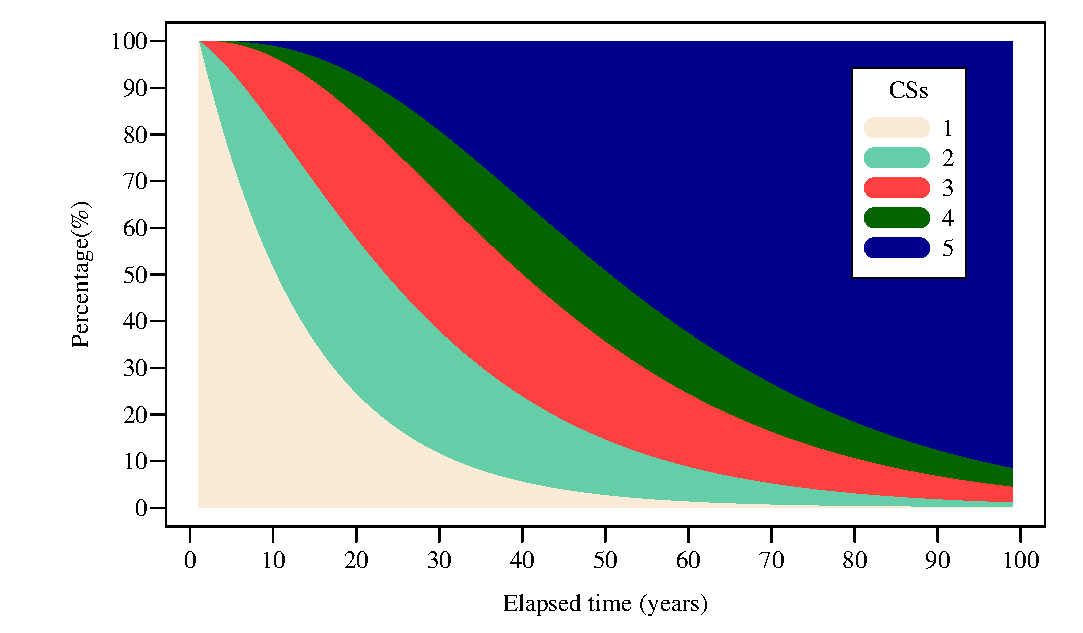
\includegraphics[scale=0.5]{pmcsdide0} \caption{Distribution of condition state over 100 years}
\label{fig:pmcsdide} 
\end{figure}

It can be seen, that it takes approximately 13 years for the deck
to move from CS1 to CS2, 17 years from CS2 to CS3, and another 16
years from CS3 to CS4 becomes, and another 12 years from CS4 to CS5.
The transition from CS1 to CS5, therefore, takes on average 58 years,
i.e. having at least one visible cracking greater than 0.5 mm.

% An example of coding (in R statistical programing language) to create proportional data using the Monte Carlo simulation techniques is given in the Github link https://github.com/namkyodai.

\subsection{Task 6: Estimate transition probabilities}

% Using the optimization model proposed in subsection \ref{optimizationmodel} on the proportional data obtained from previous task, Markov transition probability can be estimated. Table \ref{resultmtp} shows the transition probability matrix.
The transition probabilities estimated using the optimization model
proposed in subsection \ref{optimizationmodel} on the generated proportional
data are shown in matrix form in Table \ref{resultmtp}. The state
probabilities over the investigated 100 year period is shown in Figure
\ref{fig:pmcsdide-1}.
 
\begin{table}[H]
\centering \caption{{\footnotesize{}Annual Markov transition probabilities.}}
\label{resultmtp}
{\footnotesize{} }%
\begin{tabular}{c|cccccc}
\hline 
{\footnotesize{}CSs } & {\footnotesize{}1 } & {\footnotesize{}2 } & {\footnotesize{}3 } & {\footnotesize{}4 } & {\footnotesize{}5 } & \tabularnewline
\hline 
{\footnotesize{}1 } & {\footnotesize{}0.9282 } & {\footnotesize{}0.0578 } & {\footnotesize{}0.0139 } & {\footnotesize{}0.0001 } & {\footnotesize{}0.0 } & \tabularnewline
{\footnotesize{}2 } & {\footnotesize{}0.0 } & {\footnotesize{}0.9430} & {\footnotesize{}0.0570 } & {\footnotesize{}0.0 } & {\footnotesize{}0.0 } & \tabularnewline
{\footnotesize{}3 } & {\footnotesize{}0.0 } & {\footnotesize{}0.0 } & {\footnotesize{}0.9397 } & {\footnotesize{}0.0494 } & {\footnotesize{}0.0109 } & \tabularnewline
{\footnotesize{}4 } & {\footnotesize{}0.0 } & {\footnotesize{}0.0 } & {\footnotesize{}0.0 } & {\footnotesize{}0.9209 } & {\footnotesize{}0.0791 } & \tabularnewline
{\footnotesize{}5 } & {\footnotesize{}0.0 } & {\footnotesize{}0.0 } & {\footnotesize{}0.0 } & {\footnotesize{}0.0 } & {\footnotesize{}1 } & \tabularnewline
\hline 
\end{tabular}
\end{table}

% The optimization was coded in Python and published in the Github link https://github.com/hackl.
\begin{figure}[h!]
\centering 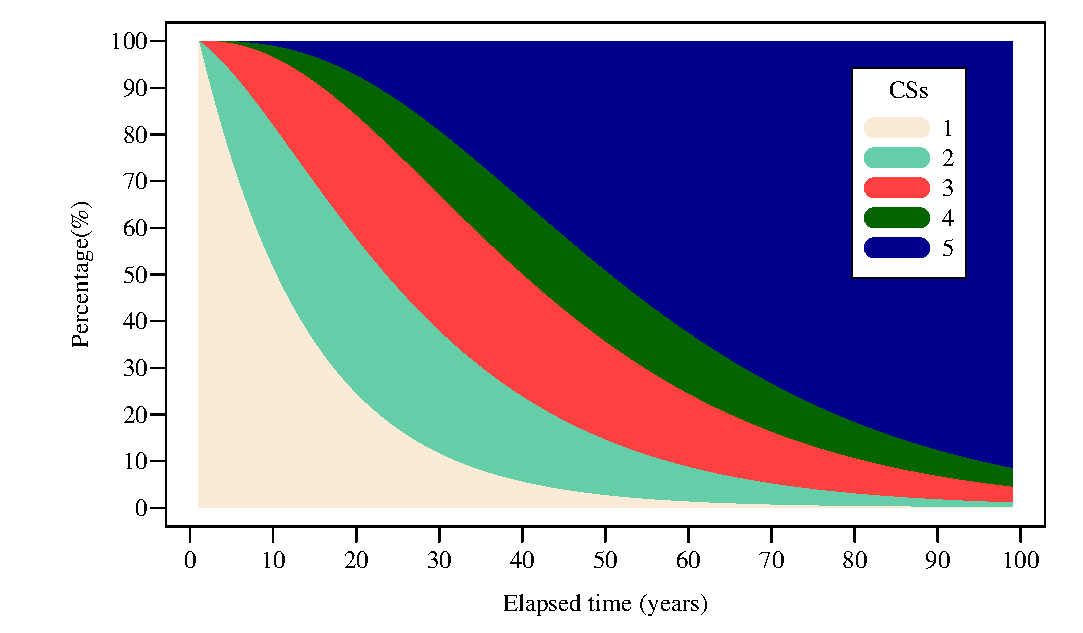
\includegraphics[scale=0.5]{pmcsdide} \caption{Distribution of condition state over 100 years}
\label{fig:pmcsdide-1} 
\end{figure}

\subsection{Task 7: Evaluation results}

It can be seen by comparing Figure \ref{fig:pmcsdide} and Figure
\ref{fig:pmcsdide-1}, predicted deterioration with the Markov model
using the estimated transition probabilities is very close to that
predicted using the mechanistic-empirical model. There is, however,
a relatively small difference between 10 to 20 years. The value of
the objective function, i.e. the minimum value of the sum of error
terms, is $-9.804887e-15$, which is extremely small. As it is small
and there are no-abnormalities in the evolution over time, the estimated
transition probabilities Table \ref{resultmtp} should be used. Noted
the optimization program used for this example was coded in Python
using the CVXPY Python-embedded modeling language for convex optimization
problems \citeN{cvxpy2016}, in which the value of control value of
residual is 0.0001, which is believed to be small enough for conversion.
The source code of the program is freely distributed on Github.

\begin{figure}[h!]
\centering 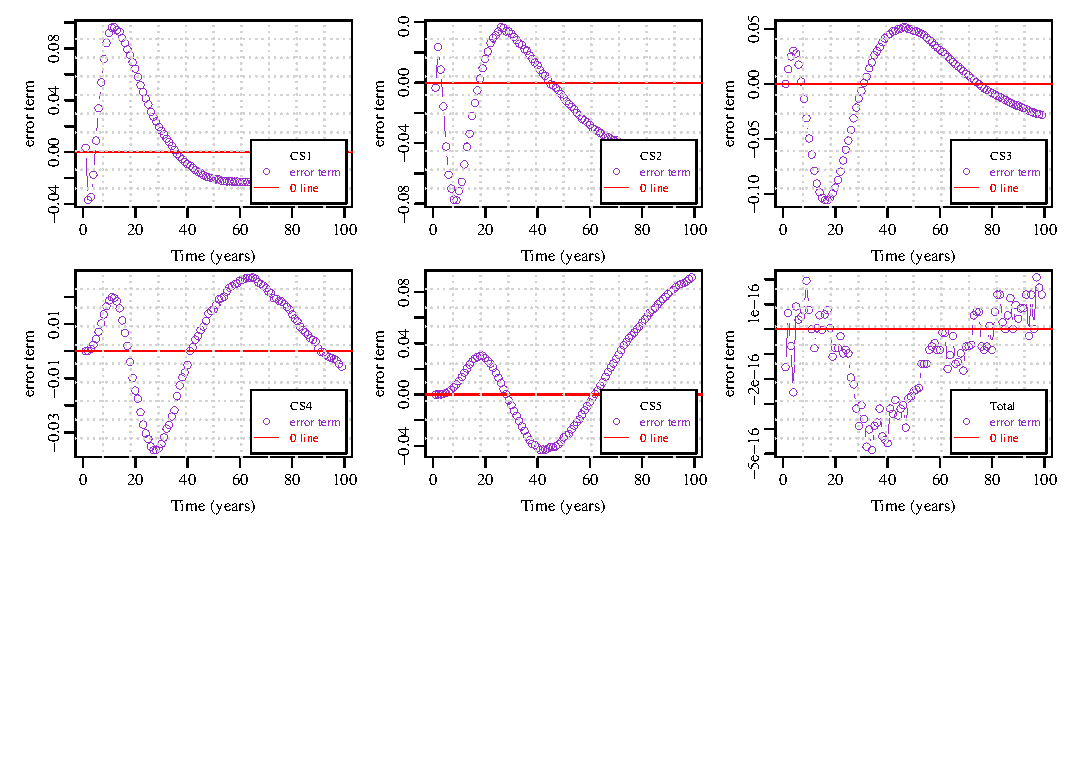
\includegraphics[scale=0.8]{evaluation} \caption{Value of error terms}


\label{evaluation} 
\end{figure}


However, when examining the error terms for each condition state at
each time step (Figure \ref{evaluation}), it can be seen that the
distributions of error terms are not stable. This instability is also
true for the total error term showing in the last graph of the figure.
This instability is most likely due to the fact that the proportional
data is generated at every time step, but the proportional data of
one time step is not dependent on the proportional data of previous
steps. 

% Overall, as indicate in the last figure of Figure \ref{evaluation},
% the sum of error terms (the value of objective function of the optimization
% model) is 3.85E-0.8, which is almost close to 0, indicating a good
% fit of obtained transition probability with the proportional data.


% % To test the stability of the transition probabilities under different set of data, the optimization model was used on reduced set of data. Each reduced set of data was proportional data corresponding to numbers of years being selected. For example, the set corresponding to 20 years mean that only the proportional data of the first 20 years was selected. Results of transition probabilities for data set corresponding to the duration of 20, 40, 60, and 80 years are shown in following tables.
% 
% \begin{table}[H]
% \footnotesize
% % \begin{center}
% \caption{Annual Markov transition probabilities (20 years proportional data).}
% \label{resultmtp20}
% \begin{tabular}{c|cccccc}\hline
% CSs & 1 & 2 & 3 & 4 & 5  \\\hline
% 1 & 0.9398  & 0.0500 & 0.0072 & 0.002 &0.001  \\
% 2 & 0.0 & 0.9743& 0.0257 & 0.0 & 0.0  \\   
% 3 &  0.0  & 0.0 & 0.9909 & 0.0091 & 0.0 \\
% 4 & 0.0 & 0.0 & 0.0  & 1.0 & 0.0  \\
% 5 &  0.0 & 0.0 & 0.0 & 0.0  & 1  \\\hline
% \end{tabular}
% % \end{center}
% \end{table}
% \begin{table}[H]
% \footnotesize
% % \begin{center}
% \caption{Annual Markov transition probabilities (40 years proportional data).}
% \label{resultmtp40}
% \begin{tabular}{c|cccccc}\hline
% CSs & 1 & 2 & 3 & 4 & 5  \\\hline
% 1 & 0.9395  & 0.0532 & 0.0069 & 0.0 &0.0004  \\
% 2 & 0.0 & 0.9611 & 0.0389 & 0.0 & 0.0  \\   
% 3 &  0.0  & 0.0 & 0.9387 & 0.0580 & 0.0033 \\
% 4 & 0.0 & 0.0 & 0.0  & 0.9037 & 0.0963  \\
% 5 &  0.0 & 0.0 & 0.0 & 0.0  & 1  \\\hline
% \end{tabular}
% % \end{center}
% \end{table}
% %
% \begin{table}[H]
% \footnotesize
% % \begin{center}
% \caption{Annual Markov transition probabilities (60 years proportional data).}
% \label{resultmtp60}
% \begin{tabular}{c|cccccc}\hline
% CSs & 1 & 2 & 3 & 4 & 5  \\\hline
% 1 & 0.9395  & 0.0531 & 0.0072 & 0.0 &0.0002  \\
% 2 & 0.0 & 0.9614& 0.0386 & 0.0 & 0.0  \\   
% 3 &  0.0  & 0.0 & 0.9364 & 0.0575 & 0.0061 \\
% 4 & 0.0 & 0.0 & 0.0  & 0.9083 & 0.0917  \\
% 5 &  0.0 & 0.0 & 0.0 & 0.0  & 1  \\\hline
% \end{tabular}
% % \end{center}
% \end{table}
% %
% \begin{table}[H]
% \footnotesize
% % \begin{center}
% \caption{Annual Markov transition probabilities (80 years proportional data).}
% \label{resultmtp80}
% \begin{tabular}{c|cccccc}\hline
% CSs & 1 & 2 & 3 & 4 & 5  \\\hline
% 1 & 0.9395  & 0.0529 & 0.0073 & 0.0001 &0.0002  \\
% 2 & 0.0 & 0.9620 & 0.0380 & 0.0 & 0.0  \\   
% 3 &  0.0  & 0.0 & 0.9371 & 0.0558 & 0.0071 \\
% 4 & 0.0 & 0.0 & 0.0  & 0.9117 & 0.0883  \\
% 5 &  0.0 & 0.0 & 0.0 & 0.0  & 1  \\\hline
% \end{tabular}
% % \end{center}
% \end{table}
% %
% It is obvious that when there are fewer numbers of yearly proportional data, the properties of transition matrix appear to have large variation in compare with that of the original data (Table \ref{resultmtp}), especially the transition probability from condition state $i$ to greater condition state $j$ ($j>i$). This is consistence with the fact that if there are less than 40 years proportional data, the transition from CS1 and CS2 to CS3, CS4, and CS5 will tend to be bias since the proportional data created are largely based on the initiation phase. In order to obtain a stable transition probability, it is recommended to create a range of proportional data for longer period of time when overseeing that the life expectancy of concrete structures can last considerably long (e.g. $>$ 60 years). 



\section{Conclusions}

\label{conclusion} In this paper, a new methodology was proposed
to estimate the transition probabilities for reinforced concrete elements
of bridges using proportional data generated from mechanistic-empirical
models. The proposed methodology makes use of a restricted least square
optimization model o determine the optimal transition probabilities.
Optimal transition probabilities are the ones that yield the minimal
total sum of error terms betweenbetween predicted distribution of
condition state in each time interval over the investigated timer
period using the Markov model and the mechanistic-empircal model directly.
The methodology was demonstrated by estimating the transition probabilities
for a reinforced concrete bridge deck. The methodology offers a way
to estimate transition probabilities when there is insufficient data
with respect to actual transitions between states, but mechanistic-empirical
models are available. A weakness of the methodology is that the distributions
of condition states in each time interval over the investigated using
the mechanistic-emrpical model is done as if the each time interval
is independent of the ones before it. Future work will be concentrated
on improving this.

% In this paper, a methodology was presented to
% estimate optimal transition probabilities to be used in Markov models
% from mechanistic-empirical models for reinforced concrete bridge elements
% deteriorating due to chloride induced corrosion of the reinforcement.
% The methodology proposes the use of two types of mechanistic-empirical
% models to create proportional data, then feeding this data into an
% optimization model to estimate the transition probability. This work
% has an important contribution to the field of bridge management as
% it proposes a way to use existing Bridge Management Systems, that
% use Markov models to predict future condition state of bridge elements,
% based on deterioration process modeled with mechanistic-empirical
% approach. The methodology was demonstrated by estimating the transition
% probabilities for a reinforced concrete bridge deck. The methodology
% offers a way to estimate transition probabilities when there is insufficient
% data with respect to actual transitions between states, but mechanistic-empirical
% models are available. 


% In this paper, a new methodology used to estimate the Markov transition probability from proportional data of reinforced concrete bridge elements has been introduced. The methodology proposes the use of two types of mechanistic-empirical models to create proportional data, then feeding this data into an optimization model to estimate the transition probability. This work has an important contribution to the field of bridge management as it proposes a way to use existing Bridge Management Systems, that use Markov models to predict future condition state of bridge elements, based on deterioration process modeled with mechanistic-empirical approach. The methodology was tested with a system of concrete deck of a bridge located in mountainous region of Switzerland. It was confirmed from the test that the methodology is feasible to be used with existing BMSs as the transition probability obtained from the optimization model became stable when proportional data of longer period of time was used. 






\pagebreak
%
%
% Here's the first appendix, the list of references:
%
\bibliography{ascexmpl}
%
% And now for some pretty impressive notation.  In this example, I have used
%   the tabular environment to line up the columns in ASCE style.
%   Note that this and all appendices (except the references) start with 
%   the \section command
%

%
\end{document}
